\documentclass[journal]{IEEEtran}

\usepackage[T1]{fontenc}
\usepackage[utf8]{inputenc}
\usepackage{graphicx}
\usepackage{amsmath}
\usepackage{booktabs}
\usepackage{hyperref}
\usepackage{tabularx}
\usepackage{array}
\usepackage{textcomp}
\usepackage{xcolor}
\usepackage{cite}
\usepackage{microtype}
\usepackage{url}

\begin{document}

\title{SSC0158 -- Arquiteturas RESTful e Boas Práticas de API}

\author{Grupo 4\\
Márcio Guilherme Vieira Silva -- 11355786\\
Rafael Jun Morita -- 10845040\\
Thiago Prado Dalla Dea -- 12691710}

\maketitle

\begin{abstract}
Este relatório apresenta um estudo empírico sobre o impacto de decisões de design em APIs RESTful no desempenho, na observabilidade e na evolutividade de aplicações distribuídas. O trabalho concentra-se em duas decisões recorrentes no desenvolvimento de APIs: o mecanismo de paginação, comparando as abordagens \textit{Offset} e \textit{Cursor}, e a estratégia de versionamento, comparando o versionamento via URI e via cabeçalhos HTTP por negociação de conteúdo. Foi implementado um protótipo funcional com FastAPI, SQLite, Docker Compose, Prometheus, Grafana, dashboard web e scripts de geração de dados e teste de carga. A API expõe rotas equivalentes para as estratégias avaliadas, permitindo a execução de experimentos controlados. Neste ciclo experimental, foram executadas 15.600 requisições HTTP em 60 execuções agregadas, com três níveis de carga, quatro alvos e cinco repetições por combinação. Os resultados incluem média, desvio padrão, intervalo de confiança de 95\%, p95, \textit{throughput} e taxa de erro.
\end{abstract}

\begin{IEEEkeywords}
REST, API, paginação, versionamento, FastAPI, Docker, Prometheus, Grafana, teste de carga.
\end{IEEEkeywords}

\section{Introdução}

A arquitetura REST (\textit{Representational State Transfer}) consolidou-se como uma das principais abordagens para construção de APIs web por combinar simplicidade, uso direto do protocolo HTTP e boa adequação a sistemas distribuídos \cite{fielding2000}. Em aplicações em nuvem, APIs RESTful frequentemente atuam como camada de comunicação entre serviços, clientes, bancos de dados e mecanismos de observabilidade. Nesse contexto, decisões aparentemente locais de projeto, como paginação de coleções ou versionamento de representações, podem influenciar desempenho, confiabilidade, manutenibilidade e evolução do sistema.

Embora REST estabeleça restrições arquiteturais gerais, a implementação concreta de uma API envolve escolhas práticas que não são completamente determinadas pelo estilo arquitetural. Entre essas escolhas, destacam-se a forma de recuperar grandes coleções de dados e a forma de evoluir representações sem quebrar clientes existentes. A paginação baseada em \textit{Offset} é simples e comum, mas pode degradar em páginas profundas porque a consulta precisa ignorar registros anteriores. Já a paginação baseada em \textit{Cursor} tende a ser mais estável para percursos progressivos, pois usa um marcador para continuar a consulta. No versionamento, o uso de URIs versionadas, como \texttt{/v1/produtos}, é direto e explícito, enquanto a negociação por cabeçalhos preserva a URI do recurso e desloca a versão para a representação desejada.

Este trabalho avalia empiricamente essas decisões por meio de uma API \textit{sandbox} de catálogo de produtos. O protótipo foi implementado em FastAPI, conteinerizado com Docker Compose e instrumentado para coleta de métricas em Prometheus. A execução experimental é apoiada por scripts de população de banco, testes de carga e visualização em dashboard web.

As principais contribuições do trabalho são:

\begin{itemize}
    \item implementação de um protótipo RESTful conteinerizado para avaliação de decisões de design;
    \item comparação experimental entre paginação \textit{Offset} e paginação \textit{Cursor};
    \item comparação experimental entre versionamento via URI e versionamento via cabeçalhos HTTP;
    \item instrumentação da API com métricas Prometheus e dashboard web simples;
    \item definição de protocolo experimental reprodutível para coleta de latência, \textit{throughput}, erros e indicadores de evolutividade.
\end{itemize}

\subsection{Definição do Problema}

APIs RESTful são amplamente utilizadas em aplicações distribuídas, mas sua qualidade depende de decisões de design tomadas durante a implementação. Mecanismos de paginação e estratégias de versionamento influenciam tanto o comportamento em tempo de execução quanto a capacidade de evolução da API.

A pergunta de pesquisa principal é:

\begin{quote}
Como decisões de design em APIs RESTful, especificamente paginação \textit{Offset} versus \textit{Cursor} e versionamento via URI versus cabeçalhos HTTP, impactam o desempenho e a evolutividade de uma API em ambiente conteinerizado?
\end{quote}


\subsection{Perguntas de Pesquisa}

A pergunta principal foi desdobrada nas seguintes perguntas de pesquisa:

\begin{itemize}
    \item \textbf{RQ1:} Como a paginação baseada em \textit{Offset} se compara à paginação baseada em \textit{Cursor} em latência, \textit{throughput}, p95 e taxa de erro sob diferentes níveis de carga?
    \item \textbf{RQ2:} O versionamento por cabeçalhos HTTP introduz custo mensurável de desempenho em relação ao versionamento via URI?
    \item \textbf{RQ3:} Quais \textit{trade-offs} de evolutividade e observabilidade surgem entre versionamento explícito por URI e negociação de conteúdo por cabeçalhos HTTP?
\end{itemize}

\subsection{Hipóteses}

\begin{itemize}
    \item \textbf{H1 (Desempenho/Paginação):} a paginação baseada em \textit{Cursor} apresentará latência mais estável em consultas a páginas profundas quando comparada à paginação baseada em \textit{Offset}.
    \item \textbf{H2 (Evolutividade/Versionamento):} o versionamento via cabeçalhos HTTP proporcionará menor acoplamento entre URI e versão da representação, facilitando a evolução da API em comparação ao versionamento explícito via URI.
\end{itemize}

\section{Trabalhos Relacionados}

O levantamento bibliográfico foi conduzido a partir de uma adaptação simplificada da metodologia PRISMA, denominada Micro-PRISMA. O objetivo foi identificar trabalhos sobre desenho, evolução, desempenho e avaliação de APIs RESTful.

\subsection{Strings de Busca e Bases}

Foram definidas as seguintes strings:

\begin{itemize}
    \item \texttt{"REST API" AND ("design" OR "anti-patterns") AND ("performance" OR "maintainability")}
    \item \texttt{"RESTful" AND "versioning" AND ("evolution" OR "maintainability")}
    \item \texttt{"REST API" AND "pagination" AND ("performance" OR "evaluation" OR "comparison")}
    \item \texttt{"RESTful API" AND "design rules" AND "empirical"}
\end{itemize}

As bases consultadas foram IEEE Xplore, ACM Digital Library, Scopus e buscas complementares em arXiv/portais dos editores para validação de metadados bibliográficos. Na triagem, foram priorizados estudos com avaliação empírica, análise de APIs reais, comparação de desempenho ou discussão direta sobre evolução/versionamento.

\subsection{Critérios de Seleção}

\begin{itemize}
    \item \textbf{Inclusão:} artigos entre 2018 e 2026; foco em APIs REST, design de APIs, evolução de APIs, desempenho sob carga ou observabilidade; disponibilidade de método, métricas ou ambiente experimental.
    \item \textbf{Exclusão:} tutoriais sem revisão técnica, textos puramente opinativos, trabalhos exclusivamente focados em segurança, estudos sem relação com APIs HTTP/REST ou sem contribuição metodológica para o projeto.
\end{itemize}

Foram identificados 45 registros iniciais. Após leitura de títulos e resumos, 12 trabalhos foram selecionados para leitura completa ou leitura técnica parcial. A Tabela \ref{tab:extracao} resume as 8 referências utilizadas diretamente na fundamentação do estudo, além da referência conceitual de Fielding usada para caracterizar o estilo REST.

\begin{table*}[htbp]
\caption{Extração de dados da literatura selecionada}
\label{tab:extracao}
\centering
\renewcommand{\arraystretch}{1.25}
\begin{tabularx}{\textwidth}{|p{3.0cm}|X|X|X|X|}
\hline
\textbf{Referência} & \textbf{Método} & \textbf{Métricas/Aspectos} & \textbf{Baseline/Comparação} & \textbf{Limitações para este trabalho} \\
\hline
Elghazal et al. \cite{elghazal2025} & Teste de carga comparativo entre modelos de APIs em contexto de microsserviços. & Tempo de resposta, eficiência de transferência e taxa de erros. & REST vs. GraphQL. & Compara modelos de API, mas não isola decisões internas de paginação e versionamento REST. \\
\hline
Gholami et al. \cite{gholami2020} & Proposta de \textit{framework} para satisfazer requisitos de desempenho em sistemas conteinerizados. & Uso de recursos, tempo de resposta e atendimento de requisitos de desempenho. & Versão única ou configuração base vs. alternativas de adaptação/versionamento. & Não foca diretamente na comparação entre paginação \textit{Offset} e \textit{Cursor}. \\
\hline
Szewczyk e Skublewska-Paszkowska \cite{szewczyk2025} & Benchmark quantitativo entre \textit{frameworks} para implementação de APIs REST. & Tempo de resposta, consumo de memória e características de implantação. & Comparação entre \textit{frameworks} REST em ambientes selecionados. & Avalia tecnologia de implementação, não decisões de modelagem de recursos. \\
\hline
Bogner et al. \cite{bogner2024} & Análise de especificações OpenAPI para identificar violações de regras RESTful. & Precisão de detecção, regras violadas e tempo de análise. & APIs aderentes vs. APIs com violações de design. & Estudo estático; não mede impacto de violações sob carga. \\
\hline
Mabotha et al. \cite{mabotha2024} & Teste de desempenho de uma API dinâmica com FastAPI, Docker e Nginx. & Tempo de resposta, \textit{throughput} e taxa de erros sob carga. & Avaliação de capacidade de uma arquitetura conteinerizada. & Não avalia variações de paginação ou versionamento como fatores experimentais. \\
\hline
Neumann et al. \cite{neumann2021} & Análise empírica de APIs REST públicas. & Aderência a princípios REST, uso de verbos HTTP, URIs, códigos de status e documentação. & Padrões REST esperados vs. implementações reais. & Foca conformidade e design observado, sem experimentos de desempenho controlados. \\
\hline
De Luca et al. \cite{deluca2026} & Estudo exploratório de \textit{anti-patterns} arquiteturais em microsserviços acadêmicos. & Incidência de \textit{anti-patterns}, impacto em escalabilidade e manutenibilidade. & Arquiteturas com e sem violações arquiteturais recorrentes. & Não quantifica isoladamente latência causada por decisões específicas de endpoints REST. \\
\hline
Kandiraju \cite{kandiraju2026} & Proposta de APIs REST de \textit{streaming} para exportação progressiva de dados relacionais. & Consumo de memória, latência de entrega e processamento incremental. & Exportação tradicional vs. recuperação progressiva por cursores. & Foca exportação de grandes volumes, não listagem paginada interativa de recursos. \\
\hline
\end{tabularx}
\end{table*}

\subsection{Lacuna Identificada}

A literatura revisada mostra que há muitos estudos sobre conformidade REST, regras de design, comparação entre modelos de API e evolução de APIs em microsserviços. Entretanto, poucos trabalhos isolam experimentalmente decisões internas de uma API REST, como paginação \textit{Offset} versus \textit{Cursor} e versionamento por URI versus cabeçalhos, em um mesmo ambiente e com métricas objetivas de desempenho e evolutividade. Este trabalho busca preencher essa lacuna por meio de uma API controlada, na qual as estratégias são implementadas lado a lado e podem ser avaliadas sob os mesmos cenários de carga.


\section{Metodologia}

A metodologia adotada combina implementação de protótipo funcional, geração controlada de dados, execução de testes de carga, coleta de métricas reais e análise quantitativa. O domínio escolhido é um catálogo de produtos, por ser simples de modelar, permitir grande volume de registros e representar uma operação comum em APIs reais: listagem paginada de recursos.

\subsection{Visão Geral da Abordagem}

O estudo foi conduzido em quatro etapas. Primeiro, foi implementada uma API RESTful \textit{sandbox} com rotas equivalentes para as decisões de design avaliadas. Segundo, foi criada uma base de dados artificial e determinística com 10.000 produtos. Terceiro, foram executados cenários controlados de carga contra os endpoints de paginação e versionamento. Por fim, os resultados foram agregados em arquivos JSON, CSV, tabelas LaTeX e gráfico SVG.

A opção por uma API \textit{sandbox} reduz interferências de regras de negócio externas e permite isolar o impacto das decisões avaliadas. Os dados de domínio são artificiais, mas os dados experimentais são reais: latências, \textit{throughput}, erros, CPU e memória foram coletados durante a execução do protótipo.

\subsection{Decisões de Design Avaliadas}

\subsubsection{Paginação}

Foram avaliadas duas estratégias. A paginação \textit{Offset} usa os parâmetros \texttt{limit} e \texttt{offset}, sendo simples de consumir e comum em APIs REST. A paginação \textit{Cursor} usa um marcador de continuidade, neste caso o identificador do último produto retornado, evitando saltos baseados em deslocamento absoluto. O experimento utilizou página profunda para enfatizar o possível custo de \textit{Offset}.

\subsubsection{Versionamento}

Foram avaliadas duas estratégias. O versionamento via URI usa caminhos explícitos, como \texttt{/v1/produtos} e \texttt{/v2/produtos}. O versionamento via cabeçalhos HTTP usa negociação de conteúdo, mantendo \texttt{/produtos} e selecionando a versão por \texttt{Accept: application/vnd.api.v2+json}. A versão \texttt{v2} adiciona o campo \texttt{meta} com \textit{timestamp}, representando uma evolução controlada da resposta.

\subsection{Baselines e Estratégias Alternativas}

\begin{itemize}
    \item \textbf{Baseline de paginação:} paginação baseada em \textit{Offset}, usando \texttt{limit} e \texttt{offset}.
    \item \textbf{Alternativa de paginação:} paginação baseada em \textit{Cursor}, usando \texttt{cursor} como marcador do último identificador retornado.
    \item \textbf{Baseline de versionamento:} versionamento via URI, usando rotas \texttt{/v1/produtos} e \texttt{/v2/produtos}.
    \item \textbf{Alternativa de versionamento:} versionamento via cabeçalhos HTTP, usando \texttt{Accept: application/vnd.api.v1+json} ou \texttt{Accept: application/vnd.api.v2+json}.
\end{itemize}

\subsection{Variáveis Independentes}

As variáveis independentes são: estratégia de paginação, estratégia de versionamento, volume de dados, nível de carga concorrente e profundidade da página consultada.

\subsection{Variáveis Dependentes}

As variáveis dependentes são: latência média, p95, \textit{throughput}, taxa de erros, uso de CPU, uso de memória e esforço de evolução. Para evolutividade, foram considerados acoplamento entre URI e versão, duplicação de rotas, compatibilidade com clientes existentes e clareza operacional.

\subsection{Métricas}

As métricas quantitativas utilizadas são:

\begin{itemize}
    \item latência média, mínima, máxima, p90, p95 e p99;
    \item \textit{throughput} em requisições por segundo;
    \item taxa de erro total e por código HTTP;
    \item uso médio e máximo de CPU do processo da API;
    \item memória residente média e máxima (RSS) do processo da API;
    \item média, desvio padrão e intervalo de confiança de 95\% para as métricas repetidas;
    \item indicadores de evolutividade: rotas necessárias, acoplamento de URI e compatibilidade de versões.
\end{itemize}

\subsection{Procedimento Experimental}

O procedimento final foi automatizado pelo script \texttt{scripts/run\_final\_experiment.py}. O script recria a base experimental, popula 10.000 produtos, inicia a API FastAPI em porta local, monitora CPU e memória do processo via \texttt{/proc}, executa o benchmark controlado e encerra o serviço ao final.

Cada combinação de cenário e alvo foi executada cinco vezes. Em cada repetição, o benchmark disparou requisições concorrentes, registrando latência, status HTTP, quantidade de erros, tempo total e \textit{throughput}. Os resultados foram exportados para \texttt{results/benchmark/raw.json}, \texttt{raw.csv}, \texttt{summary.json}, \texttt{summary.csv}, tabelas LaTeX e gráfico SVG.

\subsection{Tratamento Estatístico}

Para cada combinação de cenário e alvo, calculou-se a média das latências médias, o desvio padrão entre as cinco repetições e o intervalo de confiança de 95\%. Como cada combinação possui cinco repetições, foi usado o valor crítico \textit{t}=2,776 para quatro graus de liberdade. O p95 apresentado corresponde à média do p95 observado nas repetições.

\subsection{Critérios de Aceitação das Hipóteses}

A hipótese H1 é apoiada quando a paginação por \textit{Cursor} apresenta menor latência média, p95 mais estável, maior ou igual \textit{throughput} e taxa de erro não superior ao \textit{Offset}, especialmente sob carga alta. A hipótese H2 é apoiada quando o versionamento por cabeçalhos preserva compatibilidade e reduz o acoplamento entre URI e versão sem introduzir custo relevante de desempenho.


\section{Arquitetura do Sistema}

A arquitetura implementada tem como objetivo permitir a avaliação controlada de decisões de design em APIs RESTful. O sistema é conteinerizável, expõe aplicação web simples, coleta métricas e registra resultados exportáveis. A Figura \ref{fig:arquitetura_textual} resume os componentes.

\begin{figure*}[htbp]
\centering
\begin{minipage}{0.92\textwidth}
\footnotesize
\begin{verbatim}
+---------------------+       HTTP        +------------------------------+
| K6 / script Python  | ----------------> | FastAPI :8000                |
| testes de carga     |                   | /v1/produtos                 |
+---------------------+                   | /v1/produtos/cursor          |
                                            | /v2/produtos               |
+---------------------+       HTTP        | /v2/produtos/cursor          |
| Navegador           | ----------------> | /produtos + Accept header    |
| Dashboard web       |                   | /metrics                     |
+---------------------+                   +--------------+---------------+
                                                          |
                                                          | SQL
                                                          v
                                           +--------------+---------------+
                                           | SQLite products.db           |
                                           | volume ./data:/app/data      |
                                           +--------------+---------------+
                                                          ^
                                                          |
+---------------------+      scrape        +--------------+--------------+
| Prometheus :9090    | <---------------- | /metrics Prometheus          |
+---------------------+                   +------------------------------+
          |
          v
+---------------------+
| Grafana :3000       |
+---------------------+
\end{verbatim}
\end{minipage}
\caption{Arquitetura implementada para avaliação experimental da API RESTful.}
\label{fig:arquitetura_textual}
\end{figure*}

\subsection{Componentes}

\begin{itemize}
    \item \textbf{Protocolo de comunicação:} HTTP/REST, escolhido por aderência direta ao Tema 4 e aos objetivos de avaliar paginação, versionamento e boas práticas RESTful.
    \item \textbf{API intermediária:} aplicação FastAPI, responsável por expor endpoints REST, dashboard estático, \textit{healthcheck} e métricas Prometheus.
    \item \textbf{Banco de dados:} SQLite armazenado em volume local. A escolha reduz dependências externas e concentra o experimento nas decisões de API.
    \item \textbf{Prometheus:} coleta métricas no endpoint \texttt{/metrics}, incluindo contadores por rota/status, histograma de duração e total de produtos.
    \item \textbf{Grafana:} serviço de visualização disponível na porta 3000.
    \item \textbf{Dashboard web:} página estática servida pela API para consultar produtos, alternar estratégia de paginação, alternar versionamento e visualizar respostas JSON.
    \item \textbf{Scripts experimentais:} scripts para popular banco, executar carga, monitorar CPU/memória e exportar resultados.
\end{itemize}

\subsection{Broker e Delimitação da Trilha REST}

O enunciado da disciplina menciona broker como componente recomendado para algumas trilhas. Neste projeto, a trilha é REST e a decisão arquitetural foi manter comunicação síncrona HTTP cliente--API, sem fila assíncrona intermediária, para não misturar o fator experimental com efeitos de mensageria. Essa ausência é uma delimitação técnica do Tema 4. O arquivo Mosquitto presente no repositório foi mantido apenas como artefato de configuração não utilizado, caso uma extensão futura queira transformar a coleta de métricas em eventos publicados por broker.

\subsection{Justificativa Arquitetural}

A separação entre API, banco, scripts de carga e observabilidade torna o sistema reprodutível e próximo de uma implantação em nuvem baseada em contêineres. FastAPI foi escolhido por facilitar a criação de endpoints REST e a execução com Uvicorn. SQLite foi escolhido por simplificar a execução e reduzir variabilidade externa; essa escolha é discutida como ameaça à validade externa.


\section{Implementação}

O protótipo foi implementado no repositório com a seguinte estrutura principal:

\begin{verbatim}
├── docker-compose.yml
├── README.md
├── src/
│   ├── api.py
│   ├── Dockerfile
│   ├── requirements.txt
│   └── static/index.html
├── scripts/
│   ├── populate_db.py
│   ├── load_test_python.py
│   ├── benchmark_api.py
│   ├── run_final_experiment.py
│   └── run_experiment.sh
├── experiments/load_test.js
├── prometheus/prometheus.yml
├── tests/test_api.py
├── results/benchmark/
│   ├── raw.json
│   ├── summary.csv
│   ├── table_pagination.tex
│   ├── table_versioning.tex
│   ├── table_resources.tex
│   ├── resource_usage.csv
│   └── latency_chart.svg
└── requirements-dev.txt
\end{verbatim}

A aplicação principal está em \texttt{src/api.py}. Na inicialização, a API cria a tabela \texttt{produtos} caso ela ainda não exista. Os endpoints implementados são:

\begin{itemize}
    \item \texttt{GET /api/health}: verificação de saúde da API;
    \item \texttt{GET /metrics}: métricas no formato Prometheus;
    \item \texttt{GET /v1/produtos}: V1 com paginação \textit{Offset};
    \item \texttt{GET /v1/produtos/cursor}: V1 com paginação \textit{Cursor};
    \item \texttt{GET /v2/produtos}: V2 com paginação \textit{Offset} e campo \texttt{meta};
    \item \texttt{GET /v2/produtos/cursor}: V2 com paginação \textit{Cursor} e campo \texttt{meta};
    \item \texttt{GET /produtos}: versionamento por cabeçalho \texttt{Accept}.
\end{itemize}

O script \texttt{scripts/populate\_db.py} gera registros artificiais com campos \texttt{id}, \texttt{nome}, \texttt{categoria}, \texttt{preco}, \texttt{estoque}, \texttt{criado\_em} e \texttt{atualizado\_em}. O teste de carga principal está em \texttt{experiments/load\_test.js}, usando K6. Há também uma alternativa em Python assíncrono em \texttt{scripts/load\_test\_python.py}. Para a entrega final, o script \texttt{scripts/run\_final\_experiment.py} automatiza a execução completa: recria a base, inicia a API, monitora CPU/memória, executa o benchmark e grava os artefatos finais.

A execução básica do sistema é:

\begin{verbatim}
docker compose up -d --build
docker exec ssc0158_api python /app/scripts/populate_db.py \
  /app/data/products.db 10000
k6 run -e BASE_URL=http://localhost:8000 experiments/load_test.js
\end{verbatim}

A reprodução do experimento final usado neste relatório pode ser feita em um comando:

\begin{verbatim}
./.venv/bin/python \
  scripts/run_final_experiment.py \
  --port 8010 --products 10000 \
  --repetitions 5 \
  --output-dir results/benchmark
\end{verbatim}


\section{Configuração Experimental}

Os experimentos finais foram executados em 6 de junho de 2026 contra a API FastAPI em \texttt{http://127.0.0.1:8010}, com banco SQLite dedicado em \texttt{results/benchmark/products.db}. A base foi recriada antes da medição e populada com 10.000 produtos artificiais. A execução foi conduzida pelo script \texttt{scripts/run\_final\_experiment.py}, que inicia a API, monitora CPU/memória do processo e aciona o benchmark \texttt{scripts/benchmark\_api.py}, baseado em \texttt{httpx} assíncrono.

Cada combinação de cenário e alvo foi repetida cinco vezes. Em cada repetição, o script disparou requisições concorrentes e registrou latência, quantidade de requisições, taxa de erro, tempo total e \textit{throughput}. A Tabela \ref{tab:cenarios} descreve a carga efetivamente utilizada.

\begin{table}[htbp]
\caption{Cenários experimentais executados}
\label{tab:cenarios}
\centering
\renewcommand{\arraystretch}{1.2}
\begin{tabular}{lrrr}
\toprule
\textbf{Cenário} & \textbf{Usuários} & \textbf{Req./usuário} & \textbf{Req./repetição} \\
\midrule
C1 -- Baixa & 10 & 8 & 80 \\
C2 -- Média & 50 & 6 & 300 \\
C3 -- Alta & 100 & 4 & 400 \\
\bottomrule
\end{tabular}
\end{table}

Foram avaliados quatro alvos: paginação \textit{Offset} profunda em \texttt{/v1/produtos?limit=50\&offset=9000}, paginação \textit{Cursor} profunda em \texttt{/v1/produtos/cursor?limit=50\&cursor=9000}, versionamento via URI em \texttt{/v2/produtos?limit=50\&offset=0} e versionamento via cabeçalho em \texttt{/produtos?limit=50\&offset=0} com \texttt{Accept: application/vnd.api.v2+json}. No total, foram executadas 15.600 requisições HTTP, resultantes de 3 cenários, 4 alvos, 5 repetições e diferentes quantidades de requisições por repetição.

As métricas agregadas foram calculadas sobre as cinco repetições de cada combinação. O intervalo de confiança de 95\% foi calculado sobre a média de latência de cada repetição, usando valor crítico \textit{t} para cinco amostras. O processo da API foi amostrado 662 vezes para CPU e memória residente.


\section{Resultados Experimentais}

A Tabela \ref{tab:evidencias} resume as evidências de implementação e execução. Além dos testes unitários, os resultados brutos e processados foram armazenados em \texttt{results/benchmark/}. Os arquivos principais são \texttt{raw.json}, com as execuções individuais, \texttt{summary.csv}, com os dados agregados, \texttt{table\_pagination.tex}, \texttt{table\_versioning.tex}, \texttt{table\_resources.tex}, \texttt{resource\_usage.csv} e \texttt{latency\_chart.svg}.

\begin{table}[htbp]
\caption{Evidências experimentais do protótipo}
\label{tab:evidencias}
\centering
\renewcommand{\arraystretch}{1.2}
\begin{tabularx}{\columnwidth}{lX}
\toprule
\textbf{Evidência} & \textbf{Status} \\
\midrule
API REST & Endpoints V1, V2, cursor, offset e header implementados. \\
Banco & SQLite experimental com 10.000 produtos. \\
Dashboard & Página web consulta os endpoints reais de produtos. \\
Observabilidade & Endpoint \texttt{/metrics} expõe métricas Prometheus. \\
Testes unitários & 6 testes automatizados executados com sucesso. \\
Benchmark & 15.600 requisições HTTP, 60 execuções agregadas e 0\% de erro. \\
Resultados & JSON, CSV, tabelas LaTeX e SVG gerados em \texttt{results/benchmark/}. \\
\bottomrule
\end{tabularx}
\end{table}

\subsection{Paginação: Offset vs. Cursor}

A Tabela \ref{tab:resultados_paginacao} apresenta os resultados da comparação entre paginação \textit{Offset} e \textit{Cursor} em página profunda. A coluna ``Média'' representa a média da latência média das cinco repetições. A coluna ``DP'' representa o desvio padrão dessas médias, e ``IC95'' representa a margem do intervalo de confiança de 95\%.

\begin{table*}[htbp]
\caption{Resultados da comparação entre paginação Offset e Cursor}
\label{tab:resultados_paginacao}
\centering
\renewcommand{\arraystretch}{1.2}
\begin{tabularx}{\textwidth}{l l r r r r r r}
\toprule
\textbf{Cenário} & \textbf{Estratégia} & \textbf{Média (ms)} & \textbf{DP} & \textbf{IC95} & \textbf{p95 (ms)} & \textbf{RPS} & \textbf{Erro (\%)} \\
\midrule
C1 & Offset & 92.56 & 6.17 & 7.66 & 143.82 & 487.66 & 0.00 \\
C1 & Cursor & 84.14 & 6.57 & 8.16 & 133.32 & 519.71 & 0.00 \\
C2 & Offset & 825.19 & 19.45 & 24.15 & 1314.21 & 199.80 & 0.00 \\
C2 & Cursor & 844.58 & 21.74 & 26.99 & 1269.19 & 195.36 & 0.00 \\
C3 & Offset & 2258.78 & 34.72 & 43.11 & 3568.01 & 92.47 & 0.00 \\
C3 & Cursor & 2241.29 & 41.24 & 51.20 & 3559.47 & 93.47 & 0.00 \\
\bottomrule
\end{tabularx}
\end{table*}

A paginação \textit{Cursor} apresentou menor latência média em C1 e C3, mas não em C2. Em C1, a redução foi de aproximadamente 9,1\%; em C3, de 0,8\%. Em C2, o \textit{Offset} apresentou latência média cerca de 2,3\% menor. Apesar disso, o p95 da estratégia por \textit{Cursor} foi menor nos três cenários, sugerindo melhor comportamento nas requisições mais lentas. Como os intervalos de confiança são próximos e há inversão na média em C2, os resultados apoiam H1 de forma moderada, não conclusiva.

\subsection{Versionamento: URI vs. Cabeçalhos HTTP}

A Tabela \ref{tab:resultados_versionamento} apresenta os resultados da comparação entre versionamento via URI e via cabeçalhos HTTP. O objetivo principal dessa comparação é avaliar evolutividade, mas a medição de desempenho verifica se a negociação por cabeçalho introduz impacto perceptível na resposta.

\begin{table*}[htbp]
\caption{Resultados da comparação entre versionamento via URI e via cabeçalhos HTTP}
\label{tab:resultados_versionamento}
\centering
\renewcommand{\arraystretch}{1.2}
\begin{tabularx}{\textwidth}{l l r r r r r r}
\toprule
\textbf{Cenário} & \textbf{Estratégia} & \textbf{Média (ms)} & \textbf{DP} & \textbf{IC95} & \textbf{p95 (ms)} & \textbf{RPS} & \textbf{Erro (\%)} \\
\midrule
C1 & URI v2 & 89.48 & 4.88 & 6.06 & 142.22 & 487.55 & 0.00 \\
C1 & Header v2 & 87.61 & 2.89 & 3.59 & 137.75 & 497.58 & 0.00 \\
C2 & URI v2 & 846.79 & 40.39 & 50.15 & 1219.98 & 196.07 & 0.00 \\
C2 & Header v2 & 847.71 & 18.74 & 23.26 & 1188.20 & 195.66 & 0.00 \\
C3 & URI v2 & 2252.37 & 24.91 & 30.92 & 3730.96 & 93.07 & 0.00 \\
C3 & Header v2 & 2276.64 & 64.84 & 80.49 & 3677.21 & 92.12 & 0.00 \\
\bottomrule
\end{tabularx}
\end{table*}

Os resultados de desempenho entre URI e cabeçalhos foram próximos. Em C1, o versionamento por cabeçalho foi ligeiramente mais rápido; em C2, os valores foram praticamente equivalentes; em C3, a URI apresentou menor latência média. Em todos os casos, a taxa de erro foi 0\%. Portanto, não houve evidência de custo relevante de desempenho para a negociação por cabeçalho. A avaliação de H2 permanece principalmente arquitetural: o cabeçalho preserva a URI do recurso e reduz o acoplamento entre identificação do recurso e versão da representação, enquanto a URI versionada é mais explícita e simples de observar em logs e testes manuais.

\begin{figure*}[htbp]
\centering
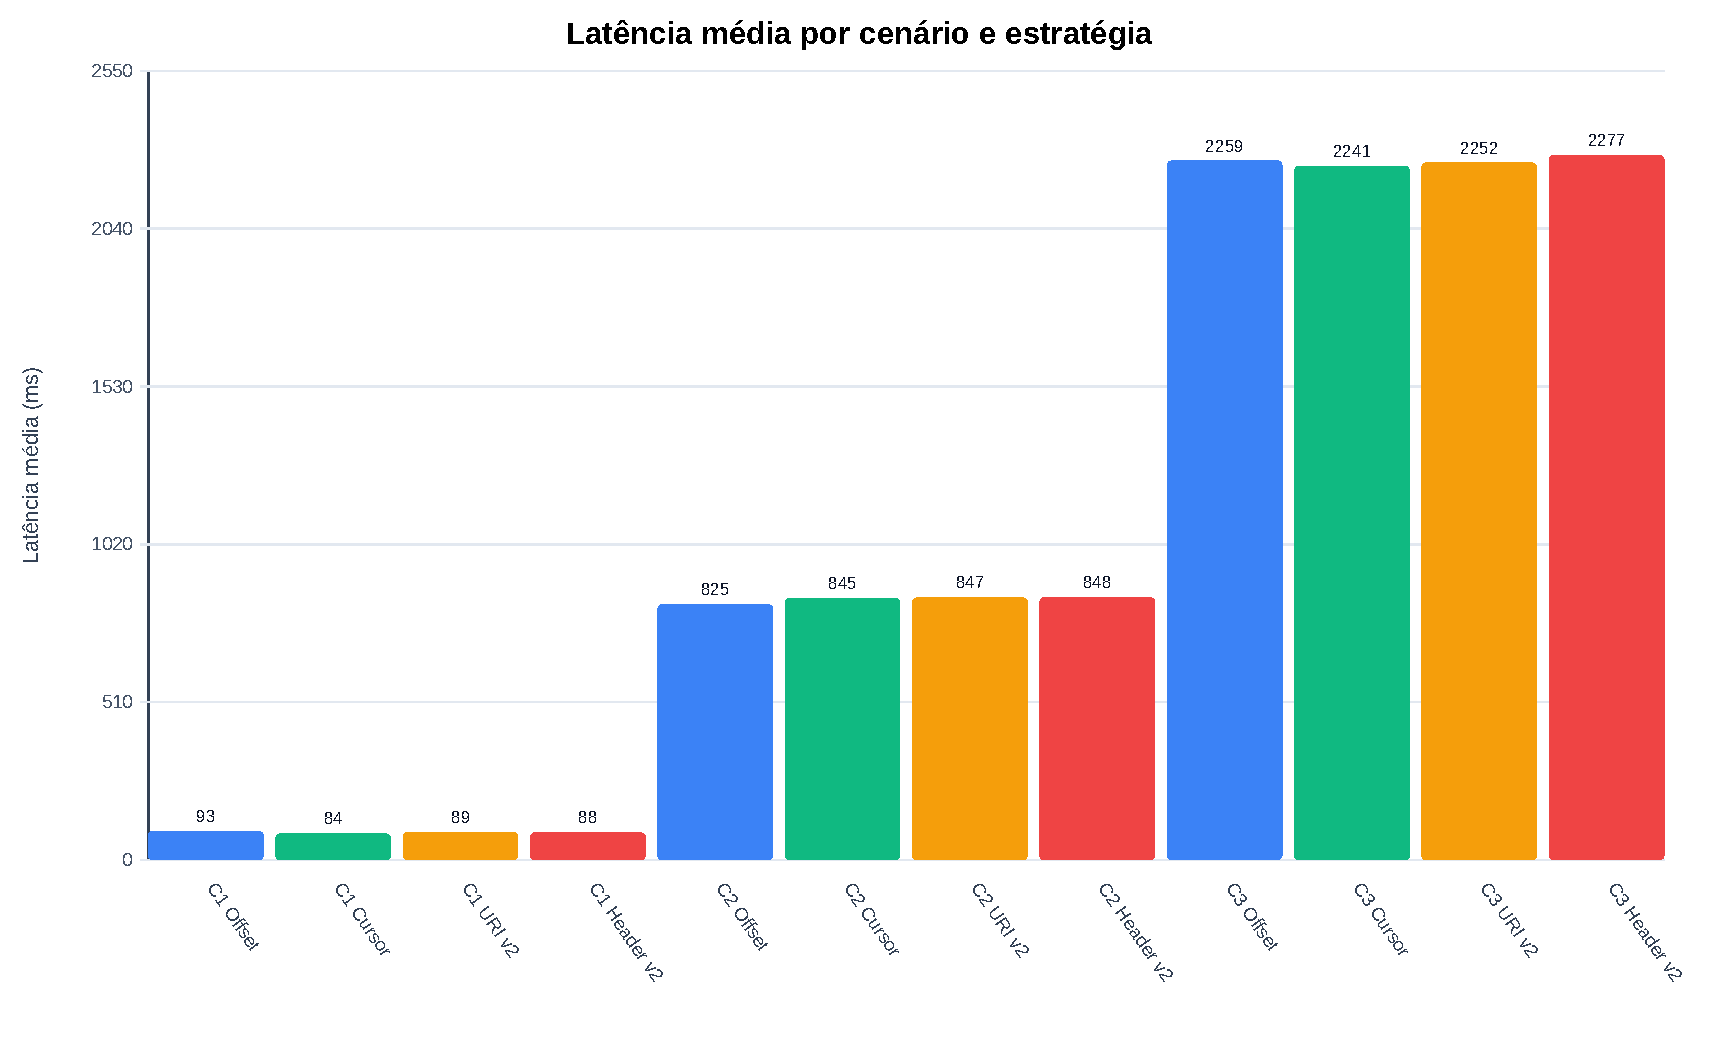
\includegraphics[width=0.95\textwidth]{figures/latency_chart.pdf}
\caption{Latência média por cenário e estratégia nos experimentos finais.}
\label{fig:latencia_media}
\end{figure*}

A Figura \ref{fig:latencia_media} reforça visualmente o crescimento de latência conforme a carga aumenta. A diferença entre estratégias permanece pequena em relação ao salto entre C1, C2 e C3, indicando que o nível de concorrência teve efeito maior sobre o tempo de resposta do que a escolha de versionamento.

\subsection{Consumo de Recursos}

Durante a execução final, o processo da API foi amostrado 662 vezes por meio de \texttt{/proc}. A Tabela \ref{tab:resultados_recursos} apresenta o uso médio e máximo de CPU e memória residente (RSS). O valor máximo de CPU pode ultrapassar 100\% porque representa uso acumulado em múltiplos núcleos lógicos durante intervalos curtos.

\begin{table*}[htbp]
\caption{Consumo de recursos observado durante o experimento final}
\label{tab:resultados_recursos}
\centering
\renewcommand{\arraystretch}{1.2}
\begin{tabularx}{\textwidth}{l r r r r r}
\toprule
\textbf{Componente} & \textbf{Amostras} & \textbf{CPU média (\%)} & \textbf{CPU máx. (\%)} & \textbf{RSS médio (MB)} & \textbf{RSS máx. (MB)} \\
\midrule
API & 662 & 37.77 & 334.44 & 72.72 & 103.94 \\
\bottomrule
\end{tabularx}
\end{table*}


\section{Discussão}

Os resultados indicam que a paginação por \textit{Cursor} apresentou vantagem em C1 e C3, além de p95 menor nos três cenários, embora a magnitude da diferença tenha sido pequena no ambiente avaliado. Isso é coerente com a expectativa teórica: em consultas profundas, a estratégia por cursor evita a semântica de descarte de registros associada ao \textit{Offset}. Entretanto, como o banco utilizado foi SQLite local, com apenas 10.000 registros e sem rede entre aplicação e banco, a diferença observada tende a ser menor do que em cenários com bancos cliente-servidor, maior cardinalidade ou consultas mais complexas.

No C3, que representa a maior carga aplicada, o \textit{Cursor} reduziu a latência média de 2258,78 ms para 2241,29 ms e elevou o \textit{throughput} médio de 92,47 para 93,47 requisições por segundo. O p95 também foi ligeiramente menor para \textit{Cursor}. Esse comportamento apoia H1 de maneira moderada: a estratégia alternativa apresentou melhor comportamento em parte das métricas, mas não com diferença grande o suficiente para ignorar a sobreposição dos intervalos de confiança e a variabilidade natural do ambiente.

Para versionamento, os resultados mostram que a escolha entre URI e cabeçalho não introduziu impacto relevante de desempenho no protótipo. A diferença deve ser interpretada principalmente em termos de evolução. A URI versionada é mais simples para clientes, documentação e inspeção manual, pois a versão está explícita no caminho. Já o cabeçalho HTTP preserva a estabilidade da URI e permite tratar a versão como uma escolha de representação, o que reduz o acoplamento conceitual entre recurso e versão. Assim, H2 é apoiada do ponto de vista arquitetural, mas não por uma diferença mensurável de latência.

A taxa de erro igual a 0\% em todos os cenários indica que a API manteve confiabilidade funcional sob as cargas aplicadas. O consumo médio de CPU foi de 37,77\%, com pico de 334,44\%, e a memória residente média foi de 72,72 MB, com pico de 103,94 MB. Esses valores indicam que o protótipo executou a carga sem esgotamento de recursos no ambiente usado, mas também mostram que a concorrência eleva rapidamente a latência quando múltiplas requisições simultâneas disputam o mesmo processo e o mesmo arquivo SQLite.


\section{Ameaças à Validade}

\subsection{Validade Interna}

Os resultados podem ser afetados por estado do cache, concorrência de processos na máquina, escalonamento do sistema operacional, aquecimento da aplicação e características do SQLite. Para mitigar essas ameaças, os cenários foram repetidos cinco vezes e os dados brutos foram preservados em \texttt{results/benchmark/raw.json}. Ainda assim, a execução local pode ter sofrido interferências de outros processos.

\subsection{Validade Externa}

O domínio de produtos é propositalmente simples. Assim, os resultados podem não generalizar diretamente para APIs com filtros complexos, \textit{joins}, autenticação, autorização, payloads maiores, bancos distribuídos ou múltiplas réplicas. A escolha por SQLite favorece reprodutibilidade, mas limita extrapolação para PostgreSQL, MySQL ou bancos distribuídos.

\subsection{Validade de Construto}

Latência, \textit{throughput}, p95 e taxa de erro são métricas adequadas para desempenho e confiabilidade, mas não capturam completamente experiência do desenvolvedor ou facilidade de manutenção. A avaliação de evolutividade combina evidência quantitativa de rotas e estrutura com análise qualitativa dos \textit{trade-offs} entre URI e cabeçalhos.

\subsection{Validade de Conclusão}

Como cada combinação foi repetida cinco vezes, o IC95 oferece uma medida inicial de incerteza, mas diferenças pequenas devem ser interpretadas com cautela. A hipótese H1 é apoiada de forma moderada, não absoluta, porque a vantagem do \textit{Cursor} não ocorreu em todas as médias. A hipótese H2 é sustentada principalmente por argumento arquitetural, e não por diferença estatística de desempenho.


\section{Checklist de Reprodutibilidade}

\begin{table}[htbp]
\caption{Checklist de reprodutibilidade}
\label{tab:checklist}
\centering
\renewcommand{\arraystretch}{1.2}
\begin{tabularx}{\columnwidth}{lX}
\toprule
\textbf{Item} & \textbf{Status} \\
\midrule
Docker/Compose & Implementado em \texttt{docker-compose.yml}. \\
Dependências fixadas & Implementado em \texttt{src/requirements.txt} e \texttt{requirements-dev.txt}. \\
README de execução & Implementado no README principal e em \texttt{relatorio/README.md}. \\
Script de população & Implementado em \texttt{scripts/populate\_db.py}. \\
Script de experimento final & Implementado em \texttt{scripts/run\_final\_experiment.py}. \\
Script de benchmark/análise & Implementado em \texttt{scripts/benchmark\_api.py}. \\
Observabilidade & Implementada com Prometheus/Grafana e \texttt{/metrics}. \\
Dashboard web & Implementado em \texttt{src/static/index.html}. \\
Resultados brutos & Implementado em \texttt{results/benchmark/raw.json}. \\
Gráficos e tabelas & Implementado em \texttt{summary.csv}, tabelas LaTeX e \texttt{latency\_chart.svg}. \\
CPU e memória & Implementado em \texttt{results/benchmark/resource\_usage.csv}. \\
Micro-PRISMA & Resumido neste relatório; planilha externa deve acompanhar a entrega, se exigida pelo docente. \\
\bottomrule
\end{tabularx}
\end{table}


\section{Conclusão}

Este relatório consolidou a proposta, a implementação e a avaliação experimental de um estudo sobre decisões de design em APIs RESTful. O protótipo desenvolvido atende ao núcleo técnico do Tema 4 da disciplina: implementa uma API RESTful conteinerizada, com estratégias alternativas de paginação e versionamento, banco de dados, dashboard web, testes automatizados, scripts de carga, coleta de métricas e observabilidade com Prometheus/Grafana.

Os experimentos executados totalizaram 15.600 requisições HTTP e não registraram erros. A paginação por \textit{Cursor} apresentou menor latência média em C1 e C3 e menor p95 nos três cenários, apoiando H1 de forma moderada. A comparação entre versionamento via URI e via cabeçalhos HTTP não indicou diferença relevante de desempenho, mas reforçou o \textit{trade-off} arquitetural de H2: URIs versionadas são mais explícitas, enquanto cabeçalhos reduzem o acoplamento entre recurso e versão da representação. O processo da API consumiu, em média, 37,77\% de CPU e 72,72 MB de memória RSS durante a execução. Como trabalhos futuros, recomenda-se repetir os testes na VM da disciplina, ampliar o volume de dados e avaliar um banco cliente-servidor, como PostgreSQL, para aumentar a validade externa dos resultados.

\appendices

\section{Resumo do Micro-PRISMA}

\begin{table}[htbp]
\caption{Resumo do processo Micro-PRISMA}
\label{tab:micro_prisma}
\centering
\renewcommand{\arraystretch}{1.2}
\begin{tabularx}{\columnwidth}{l r X}
\toprule
\textbf{Etapa} & \textbf{Qtd.} & \textbf{Descrição} \\
\midrule
Identificação & 45 & Registros obtidos com quatro strings em IEEE Xplore, ACM Digital Library, Scopus e buscas complementares. \\
Triagem & 12 & Trabalhos selecionados por título e resumo para leitura completa ou parcial. \\
Inclusão final & 8 & Estudos diretamente usados na tabela de extração e fundamentação. \\
\bottomrule
\end{tabularx}
\end{table}

Os critérios de inclusão priorizaram estudos empíricos ou metodológicos relacionados a APIs REST, desempenho, evolução, versionamento, boas práticas e observabilidade. Os critérios de exclusão removeram textos opinativos, tutoriais, trabalhos sem relação direta com REST/HTTP e estudos exclusivamente focados em segurança. A lacuna identificada foi a baixa quantidade de estudos que isolam experimentalmente decisões internas de design REST, como paginação e versionamento, em um mesmo ambiente controlado.

\section{Artefatos de Reprodutibilidade}

Os principais artefatos para reprodução são: \texttt{docker-compose.yml}, \texttt{src/Dockerfile}, \texttt{src/requirements.txt}, \texttt{requirements-dev.txt}, \texttt{scripts/populate\_db.py}, \texttt{scripts/benchmark\_api.py}, \texttt{scripts/run\_final\_experiment.py}, \texttt{experiments/load\_test.js}, \texttt{prometheus/prometheus.yml} e o diretório \texttt{results/benchmark/}. O comando recomendado para reproduzir a rodada final é:

\begin{verbatim}
  ./.venv/bin/python \
  scripts/run_final_experiment.py \
  --port 8010 --products 10000 \
  --repetitions 5 \
  --output-dir results/benchmark
\end{verbatim}

A geração dos produtos é determinística em função do índice \texttt{i}; portanto, não há semente aleatória a controlar. Os metadados de execução ficam registrados em \texttt{summary.json} e \texttt{resource\_usage.json}.

\bibliographystyle{IEEEtran}
\bibliography{references}

\end{document}
